%==============================================================================
% SHARED ELEMENTS: Reusable Figures, Tables, Equations
%==============================================================================
% Define once, use in both report and presentation

%------------------------------------------------------------------------------
% CUSTOM COMMANDS
%------------------------------------------------------------------------------
\newcommand{\keyword}[1]{\textbf{#1}}
\newcommand{\term}[1]{\textit{#1}}

%==============================================================================
% FIGURES (define as commands)
%==============================================================================

% Example: Temperature plot
\newcommand{\figureTempData}{
    % TikZ/PGFPlots figure - Temperature vs Time
% This file is included directly in the LaTeX document
% To compile standalone: pdflatex -jobname=sample_plot "\documentclass{standalone}\usepackage{pgfplots}\begin{document}% TikZ/PGFPlots figure - Temperature vs Time
% This file is included directly in the LaTeX document
% To compile standalone: pdflatex -jobname=sample_plot "\documentclass{standalone}\usepackage{pgfplots}\begin{document}% TikZ/PGFPlots figure - Temperature vs Time
% This file is included directly in the LaTeX document
% To compile standalone: pdflatex -jobname=sample_plot "\documentclass{standalone}\usepackage{pgfplots}\begin{document}\input{sample_plot.tex}\end{document}"

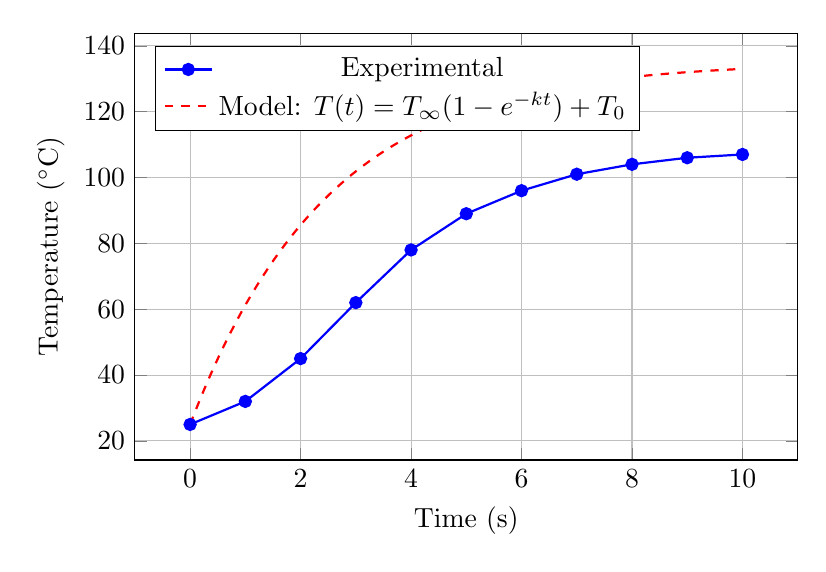
\begin{tikzpicture}
    \begin{axis}[
        width=10cm,
        height=7cm,
        xlabel={Time (s)},
        ylabel={Temperature ($^\circ$C)},
        grid=major,
        legend pos=north west,
        ylabel near ticks,
        xlabel near ticks
    ]
    
    % Sample data - exponential heating curve
    \addplot[blue, thick, mark=*, mark size=2pt] coordinates {
        (0, 25) (1, 32) (2, 45) (3, 62) (4, 78) 
        (5, 89) (6, 96) (7, 101) (8, 104) (9, 106) (10, 107)
    };
    \addlegendentry{Experimental}
    
    % Theoretical curve
    \addplot[red, thick, dashed, domain=0:10, samples=100] 
        {110*(1-exp(-0.4*x)) + 25};
    \addlegendentry{Model: $T(t) = T_{\infty}(1-e^{-kt}) + T_0$}
    
    \end{axis}
\end{tikzpicture}
\end{document}"

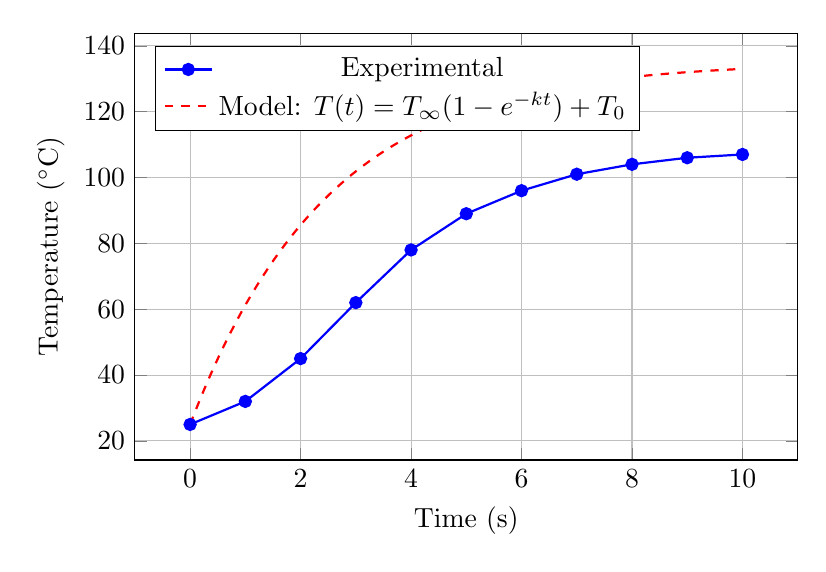
\begin{tikzpicture}
    \begin{axis}[
        width=10cm,
        height=7cm,
        xlabel={Time (s)},
        ylabel={Temperature ($^\circ$C)},
        grid=major,
        legend pos=north west,
        ylabel near ticks,
        xlabel near ticks
    ]
    
    % Sample data - exponential heating curve
    \addplot[blue, thick, mark=*, mark size=2pt] coordinates {
        (0, 25) (1, 32) (2, 45) (3, 62) (4, 78) 
        (5, 89) (6, 96) (7, 101) (8, 104) (9, 106) (10, 107)
    };
    \addlegendentry{Experimental}
    
    % Theoretical curve
    \addplot[red, thick, dashed, domain=0:10, samples=100] 
        {110*(1-exp(-0.4*x)) + 25};
    \addlegendentry{Model: $T(t) = T_{\infty}(1-e^{-kt}) + T_0$}
    
    \end{axis}
\end{tikzpicture}
\end{document}"

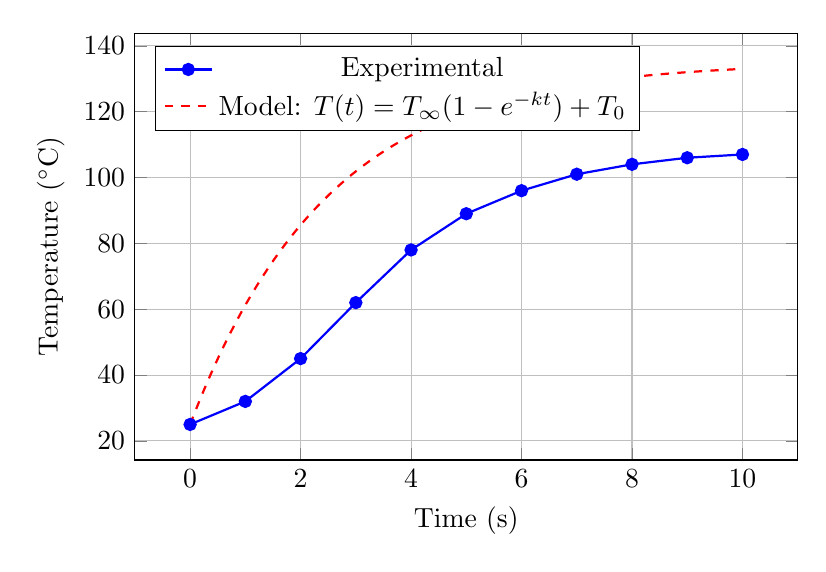
\begin{tikzpicture}
    \begin{axis}[
        width=10cm,
        height=7cm,
        xlabel={Time (s)},
        ylabel={Temperature ($^\circ$C)},
        grid=major,
        legend pos=north west,
        ylabel near ticks,
        xlabel near ticks
    ]
    
    % Sample data - exponential heating curve
    \addplot[blue, thick, mark=*, mark size=2pt] coordinates {
        (0, 25) (1, 32) (2, 45) (3, 62) (4, 78) 
        (5, 89) (6, 96) (7, 101) (8, 104) (9, 106) (10, 107)
    };
    \addlegendentry{Experimental}
    
    % Theoretical curve
    \addplot[red, thick, dashed, domain=0:10, samples=100] 
        {110*(1-exp(-0.4*x)) + 25};
    \addlegendentry{Model: $T(t) = T_{\infty}(1-e^{-kt}) + T_0$}
    
    \end{axis}
\end{tikzpicture}

}

% Usage in report:
%   \begin{figure}[htbp]
%       \centering
%       \figureTempData
%       \caption{...}
%       \label{fig:temp}
%   \end{figure}
%
% Usage in presentation:
%   \begin{frame}{Results}
%       \begin{center}
%           \scalebox{0.8}{\figureTempData}
%       \end{center}
%   \end{frame}

% Add more figures:
% \newcommand{\figureSecondary}{\includegraphics[width=0.7\textwidth]{figures/plot2.png}}

%==============================================================================
% TABLES (define as commands)
%==============================================================================

\newcommand{\tableResults}{
    \begin{tabular}{lcccc}
        \hline
        \textbf{Method} & \textbf{Metric 1} & \textbf{Metric 2} & \textbf{Metric 3} & \textbf{Overall} \\
        \hline
        Approach A      & 0.85 & 0.92 & 0.78 & 85.0 \\
        Approach B      & 0.90 & 0.88 & 0.82 & 86.7 \\
        Approach C      & 0.82 & 0.95 & 0.80 & 85.7 \\
        \textbf{Proposed} & \textbf{0.93} & \textbf{0.94} & \textbf{0.89} & \textbf{92.0} \\
        \hline
    \end{tabular}
}

% Usage in report: \begin{table}...\tableResults...\end{table}
% Usage in presentation: \begin{frame}...\small\tableResults...\end{frame}

%==============================================================================
% EQUATIONS (define as commands)
%==============================================================================

\newcommand{\eqThermalResponse}{
    T(t) = T_{\infty}(1 - e^{-kt}) + T_0 e^{-kt}
}

% Usage in report: \begin{equation} \eqThermalResponse \label{eq:thermal} \end{equation}
% Usage in presentation: $\eqThermalResponse$ or \begin{equation*} \eqThermalResponse \end{equation*}

% Add more equations:
% \newcommand{\eqObjective}{J(\theta) = \sum_{i=1}^{N} (y_i - \hat{y}_i)^2}

%------------------------------------------------------------------------------
% PARAMETERS (with math mode)
%------------------------------------------------------------------------------
\newcommand{\thermalConstant}{$k = 0.40\,\text{s}^{-1}$}
\newcommand{\ambientTemp}{$T_{\infty} = 110^{\circ}\text{C}$}
\newcommand{\initialTemp}{$T_0 = 25^{\circ}\text{C}$}

% Usage: "The time constant \thermalConstant was extracted from the fit."
% Add more: \newcommand{\sampleSize}{$N = 100$}
